\documentclass[a4paper]{article}

\usepackage{epsfig}

\newcommand{\freehep}{\textsf{FreeHEP}}
\newcommand{\class}[1]{\texttt{#1}}
\newcommand{\fhclass}[1]{\class{#1}}
\newcommand{\method}[1]{\textsf{#1}}
\newcommand{\code}[1]{\texttt{#1}}
\newcommand{\techterm}[1]{\textit{#1}}
\newcommand{\ps}{PostScript}
\newcommand{\pdf}{PDF}
\newcommand{\booktitle}[1]{\textit{#1}}
\newcommand{\syntax}[1]{\textsf{#1}}

\title{%
  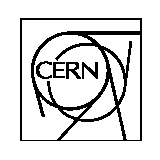
\epsfig{file=cern.eps,height=35pt}%
  \hspace{5pt}%
  \parbox[b]{9cm}{%
    \flushleft{Improvements to the \fhclass{graphics2d} package of the
      \freehep{}\footnote{\texttt{http://www.freehep.org}} Java library}
    }
  }

\author{
  Mark D\"onszelmann\footnote{CERN, Geneva, Switzerland,
    \texttt{Mark.Donszelmann@cern.ch}},
  Simon Fischer%
  \footnote{University of Dortmund, Germany,
    \texttt{simon@united-wizards.de}} and
  Sami Kama%
  \footnote{Middle East Technical University, Ankara, Turkey,
    \texttt{sami\_kama@yahoo.com}}
  }

\begin{document}


\maketitle


\abstract{This report summarises the improvements made to the
  \fhclass{graphics2d} package of the \freehep{} open source Java
  library within the scope of the Summer Student Programme 2001 of the
  European Organisation for Nuclear Research
  (CERN). A new \pdf{} driver
  was written and classes for embedding Type 1 and Type 3 fonts were
  introduced.}


\tableofcontents





\section{Introduction}

The \freehep{} \fhclass{graphics2d} package provides a set of output
drivers for vector oriented document formats among which are the
portable document format (\pdf{}), Encapsulated PostScript (EPS) and
scalable vector graphics (SVG). The latter is mainly used for the
world wide web. A special \fhclass{PixelGraphics} implementation can
be used to render to the screen. Compared to screen dumps, vector
oriented formats have the advantage of retaining their high precision
at any scale. This is especially valuable when rendering to a high
resolution device, for instance a printer.

The \fhclass{graphics2d} package is designed to be easily pluggable
into existing applications. It is therefore resembles the Java
graphics classes.





\section{Features}

\subsection{Class hierarchy}

The class hierarchy (see figure \ref{classes}) of the \freehep{} graphics2d package adopts the
Java graphics context class hierarchy. Parallel to the abstract graphics context
classes \class{Graphics} and \class{Graphics2D} that come with Java
1.1 and 1.2, there are two interfaces \fhclass{VectorGraphics1} and
\fhclass{VectorGra\-phics2} which declare methods that are guaranteed to
work with the respective Java versions. Among these are all methods
known to Java plus methods to implement some features that will be focussed on in the
next section. Finally there are the abstract classes
\fhclass{VectorGraphics} (not shown) and \fhclass{VectorGraphics2D},
each of which implements one of the interfaces and extends one of
Java's graphics contexts. They contain default implementations for
some methods, where this is possible, plus the wrappers from integer
to double methods. All actual graphics drivers for the various output
formats inherit from one of these classes. The drivers for \ps{} and
\pdf{} are described in \ref{pdfg2d} and \ref{psg2d}.

\begin{figure}[htbo]
\center{\epsfig{file=classes.eps}}
\caption{The \fhclass{graphics2d} inheritance tree}
\label{classes}
\end{figure}


\subsection{Overview of the \fhclass{VectorGraphics2D} Features}

Being a subclass of \class{Graphics2D}, \fhclass{VectorGraphics2D}
inherits all methods for drawing of lines, shapes, and text,
setting of strokes, paints, and fonts, and transformations. Additionally
all drawing methods are available in double precision. These methods
require no further discussion. See \cite{java2d} and \cite{javaapi}
for details.

\subsubsection{Additional features}

In addition to the standard Java features there are some handy
methods especially interesting for applications in high energy
physics.

Displaying a physics event might easily require some thousand tiny
boxes, triangles or circles. The method \method{drawSymbol()} renders
these symbols at high performance and lower filesize.

In order to format text on a diagram, one does not need a complex text
layout system. \freehep{} chooses the approach of limited HTML strings
which can be used to format the text while drawing. Tags are available
for italic, bold, typewriter, superscript, subscript, underline, and
overline text. Furthermore strings can be underlaid by banners and
surrounded by boxes.

\subsubsection{Multi page documents}

Some of the output drivers additionally implement the
\fhclass{MultipageDocument} interface which, as one can easily guess,
facilitates output documents containing a set of graphics each of which
is drawn on a separate page. The only thing to do is to frame the drawing
of the page by invoking \method{openPage()} and \method{closePage()}.

\subsubsection{Drawing to a \fhclass{VectorGraphics2D} context}

\ps{} and \pdf{} files have a special stack-based file organisation. The
paint, stroke, transformation, clipping area, and font altogether form
the \techterm{graphics state}. Some of the output formats might
allow only the modification of these parameters but not their direct
setting. Such a modification might be the intersection of the clipping
area or a concatenation of the current transformation matrix.  
Due to this, a special approach for drawing on \fhclass{VectorGraphics}
contexts is highly recommended.
\label{createdispose}
First one creates a new graphics context as a copy of the existing
graphics state by calling \method{create()}. Then one draws on it
narrowing down the clipping area or making arbitrary transformations
if desired, thereby changing the current graphics state. Finally one
disposes of the newly created graphics context by calling
\method{dispose()} and continues drawing on the original context using
the previous graphics state.



\subsection{The new \fhclass{PDFGraphics2D} driver}
\label{pdfg2d}

\subsubsection{Features}
%% Explain sentence
As \pdf{} is a quite powerful format the \pdf{} driver supports almost all
features. It facilitates multi page output and embedded
thumbnails as well as bookmarks for easy navigation within the
document. Fonts can be embedded either as Type1 or Type3.


\subsubsection{Implementation}
The \pdf{} driver was written from scratch along the lines of the
existing \ps{} driver. \pdf{} files \cite{pdfref} are
organised in a tree-like structure consisting mainly of dictionaries
and streams. A page dictionary might reference another dictionary
describing the required resources and  a stream containing the
contents of the page. This stream might again reference an image, stored as a so
called \techterm{XObject} in a separate stream. The actual page
contents consist of a set of commands for constructing and filling
paths, showing text, and many more.

In order to write syntactically correct \pdf{} output, utilities from
the \fhclass{org.freehep.util.pdf} package were used. The main class
\fhclass{PDFWriter} has a set of methods to open and close
dictionaries, streams, and objects. It counts byte offsets and
lengths of these objects and keeps track of references. These values
are needed for the reference table at the end of a \pdf file.

Additional utility classes for delaying the writing of objects like
images and patterns to the end of the page stream were introduced and
added to the package.


\subsection{Newly implemented features of \fhclass{PSGraphics2D}}
\label{psg2d}
Some improvements have been made to the \ps{} \cite{psref}
driver. Apart from some minor changes like adding support for shading
patterns, there are two major changes. \fhclass{PSGraphics2D} now
implements the \fhclass{Multi\-page\-Docu\-ment} interface and is capable of
embedding Type1 and Type3 fonts.





\section{Using the library}

Generally the usage of the library does not require any changes to
existing code. As the \fhclass{VectorGraphics2D} subclasses extend
\class{Graphics} as well, they can be used as an argument to the
\method{paint()} method of any component.

\subsection{Creation of and drawing on graphics contexts}

In order to make use of the additional features, one has to use the
\fhclass{Vec\-tor\-Gra\-phics} interface. This section gives an
example how to do this.

It is possible to create a document independent of any panel or
frame. It can simply be created by a constructor or factory method and
prepared for drawing onto it by making the desired settings with the
respective methds. After drawing onto the context, the file can finally
be closed. See the javadoc of \fhclass{VectorGraphics2D} and its subclasses
for details \cite{fhjavadoc}.

More probably you will want to use \fhclass{VectorGraphics2} in the
context of a \class{JPanel} or a similar component. Therefore you
should override the component's \method{paint()} or \method{print()}
method and create a \fhclass{VectorGraphics2} instance as shown in
the following example.
\medskip

\begin{verbatim}
public void paintComponent(Graphics g) {
  if (g != null) {
    // create a VectorGraphics2 instance
    VectorGrahpics2 vg = 
      VectorGraphicsUtilities2.makeVectorGraphics2(g);
    // paint your graphics
    vg.drawSymbol(90, 105, 10, 
                  VectorGraphicsConstants.SYMBOL_UP_TRIANGLE);
    vg.drawString(new TagString("Hello <b>World</b>!"), 
                  100, 100);
  } 
}
\end{verbatim}
\medskip

\noindent
When you draw to the graphics context keep in mind to use
\method{create()} and \method{dispose()} as described in
\ref{createdispose}. Notice that the factory method used will produce
a \fhclass{PixelGraphics2D} to display graphics on the screen in case
\code{g} is a standard Java graphics context. If \code{g} already is a
\fhclass{VectorGraphics2}, for instance \fhclass{PDFGraphics2D} it will
simply return \code{g} itself.


\subsection{Exporting components to a file}

An easy way of exporting components is provided by the
\fhclass{ExportDialog}. It brings up a file chooser and lets the user
select a format to save a given component or array of components in.
\medskip

\begin{verbatim}
public class ExportFrame extends JFrame {

    private ExportDialog dialog;
    private JComponent contents;

    public ExportFrame() {
        super("Export Frame");

        dialog = new ExportDialog();
        dialog.addExportFileType(new PDF2DExportFileType());
        // ... add ps, eps, svg, gif,...

        // [...] initialize the component "contents", which
        // is to be exported, here and add it to the frame
        getContentPane().add(contents);
    }

    // call this method when an appropriate event is fired
    public void export() {
      dialog.showExportDialog(this, contents);
    }
}
\end{verbatim}
\medskip
%% ADD: snapshot

\noindent
The \method{showExportDialog()} method will bring up a dialog which
lets the user choose a format and a file. Then it will create an
appropriate graphics driver and use it as the argument to the
\method{paint()} method of \code{content} to produce the output.



\section{Font embedding}


A font is a program that defines a particular shape (glyph) for every
character in a character set. In order for a  program to be able to
display a given text properly it is necessary to access these
fonts. Usually there are several fonts installed in a system. But
sometimes, especially when transferring the documents between
different computers, a processing program might not be able to find the
necessary fonts. In order to prevent this, one must be sure
about the existence of  the necessary fonts. One way to do this is
embedding the font
into the document itself. Embedding a font into a document needs
special encoding depending on the type of the document, font type and
system type. In the \freehep{} graphics2D package this is done by several
classes. \fhclass{FontIncluder} is abstract superclass of all font embedding
classes. It is extended by the \fhclass{FontEmbedder} class, which is the superclass
of several type font embedding classes. See figure \ref{fontclasses}. 

\begin{figure}[htbo]
\center{\epsfig{file=fontembedding.eps,width=10cm}}
\caption{The font embedder inheritance tree}
\label{fontclasses}
\end{figure}

These classes are used for extracting the data from the Java and
putting them into font formats supported by \ps{} and \pdf{}. Usually
fonts are divided into two main section an Encoding array, which is a
mapping between character values and shape definitions, and a glyph
dictionary that contains necessary information for drawing the
shapes. To show a character, a processing program follows the
procedure shown in figure \ref{encoding}. The argument to the text
showing operator is a string. Actually this string consists of a set
of bytes, specifying the character codes. Looking up their unique unicode
names in the encoding table, the application can use these as keys for
the glyph table and finally retrieve the characters shapes.

\begin{figure}[htbo]
\center{\epsfig{file=encoding.eps,width=10cm}}
\caption{Encoding scheme}
\label{encoding}
\end{figure}

Since we are getting the information from Java and since it uses
unicode, having different Encoding array, we must generate the
Encoding array ourselves.


\subsection{Encoding}

To get the proper encoding arrays for a font, the \fhclass{Lookup} class is
used. \fhclass{Lookup} class holds several \fhclass{CharTable} classes
, which are generated by the \fhclass{CharTableGenerator} class from a
set of definition files\ref{ctgen}. One can get the necessary
\fhclass{CharTable} class for a specific font from the
\fhclass{Lookup} class. The \fhclass{CharTable} instances contain
character names, the encoding array and unicode numbers of the characters
of that font. Once one has the unicode number, name and the encoding
of a character one can get the shape of that character from
Java. Having all necessary information the font can embedded into the
document. Currently Type 1
and Type 3 fonts are supported. The Encoding array of a font is
constructed by looping over all possible character codes and
calling the  \method{toName()} method of the proper
\fhclass{CharTable} instance. After the Encoding array is created, it can
be used to generate the simpler Type 3 fonts or the more complicated
Type 1 fonts.

\begin{figure}[htbo]
\center{\epsfig{file=ctgen.eps}}
\caption{Generation of CharTables}
\label{ctgen}
\end{figure}


\subsection{Type 3 fonts}

Type 3 fonts are \ps{} programs that are written in clear text. In
Type 3 fonts shapes are constructed with standard \ps{} operators such as
curveto, lineto, fill, moveto, etc. This property makes them easy to
construct and understand. However, since they are not encoded in any way, they
consume more space than the Type 1 fonts. Type 3 font embedding is
handled by \fhclass{FontEmbedderPDFType3} for \pdf{} files and \fhclass{FontEmbedderPS} for
\ps{} files. Both classes start processing with a chartable which they
got from the \fhclass{Lookup} class, generate the Encoding array and
the \syntax{CharProcs} dictionary, which contains glyph definitions as
\ps{} procedures. \fhclass{FontEmbedderPS} also generates a
\syntax{Metric} array to set the font advances widths properly. Finally
both \fhclass{FontEmbedderPS} and  \fhclass{FontEmbedderPDFType3} put
the created font into the document in proper formatting for the
document type.


\subsection{Type 1 fonts}

Type 1 \cite{type1} fonts are a special case of a \ps{} program. It
contains both a clear text part and an encoded-encrypted part. It also
contains \techterm{hints} to preserve character shapes to some extend in
extreme cases, e.g. at small sizes. Type 1 font embedding is done by the
\fhclass{FontEmbedderType1}
class for both \pdf{} and \ps{} files, since both formats can handle
Type 1 fonts. \fhclass{FontEmbedderType1} uses several
utility classes to generate the encoded part of the font file. These
are the \fhclass{CharStringEncoder} and the \fhclass{EEXECEncryption}
utility classes. First the \fhclass{FontEmbedderType1} class gets
the proper \fhclass{CharTable} instance from \fhclass{Lookup} with a
\method{getTable()} call and constructs the Encoding array. Then, from 
the names in the encoding array it constructs the \syntax{CharProcs}
dictionary. Subsequently it sends the \syntax{CharProcs} dictionary
through \fhclass{CharStringEncoder} and \fhclass{EEXECEncryption}
classes to encode and encrypt the dictionary. Finally it sends all
data to the proper output stream. However these classes do not support
hints yet, because Java does not contain hint information. One could
get that information from a TrueTypeFont file.


\subsection{TrueType Fonts}

In order to obtain the necessary font description we can use two
sources of information. Using the standard Java \class{Font} and
\class{GlyphVector} classes one can easily get the glyphs'
shapes. Getting the hints for the glyphs is more difficult. TrueType
font files \cite{ttf}, which are organised in tables, contain this
information. The tables can be retrieved via Java's \class{OpenType}
interface by their names as uninterpreted byte arrays. Unfortunately
no font implements this interface yet. Therefore the \fhclass{TTFFile}
class can read a TrueType font from a file and should (which we cannot
test yet) be able to read them from the \class{OpenType} data as
well. Subclasses of \fhclass{TTFTable} contain all the interpreted
data available in the TrueType font.

Since JDK 1.3 Java is shipped with some Lucida fonts which are
in TrueType format. As of JDK 1.4 these fonts also include hints.





\section{Conclusion}

The \fhclass{VectorGraphics} interfaces proved to be very suitable to
build further output drivers upon. It was possible to implement
all features for the \pdf{} driver within a short time. Redundancy
between the old and new drivers was taken as an occasion 
to do some refactoring. Methods were moved up in the class hierarchy
or to utility classes. The generated output including Type1 and Type3
fonts was tested with several versions of Adobe Acrobat Reader,
Ghostview and Ghostscript and displays properly. The work was
completed within eleven weeks.

The \fhclass{graphics2d} package, as well as the entire \freehep{}
library, can be used in a wide field of applications. The improvements
done are tested with the WIRED\footnote{http://wired.cern.ch/}
event display plug-in for JAS\footnote{http://jas.freehep.org} and
work fine. It should be no problem to include the library in existing
software projects.

\bigskip

\noindent
There are still some things that need to be done.
\begin{itemize}
\item Check the next Java version for \class{OpenType} implementations
  and check whether or not the \fhclass{TTFTable} implementations read
  them correctly
\item Add TrueType font embedding
\item Complete some minor features in the graphics drivers like
  cyclic gradients fill for \pdf{} and image tiling for \ps{}
\end{itemize}





\section{Acknowledgements}

We like to thank Charles Loomis, who built the fundaments of the
\fhclass{graphics2d} package, designed its interfaces, and class
hierarchy and implemented the \ps{} drivers.






\begin{thebibliography}{99}
\bibitem{java2d}Satyaraj Pantham: \booktitle{JFC 2D Graphics and
  Imaging}, SAMS, 2000
\bibitem{javaapi}\booktitle{Java 2 Platform, Standard Edition, v 1.3.1
  API Specification}
  \texttt{http://java.sun.com/j2se/docs/api/index.html}
\bibitem{pdfref}Jim Meehan, Ed Taft, Steve Chernicoff, Caroline Rose:
  \booktitle{PDF reference, version 1.3}, 2nd ed., Addison Wesley (2000)
\bibitem{psref}Ed Taft, Steve Chernicoff, Caroline Rose:
  \booktitle{PostScript language reference}, 3rd ed., Addison Wesley
  (1999)
\bibitem{fhjavadoc}\booktitle{FreeHEP Overview}
  \texttt{http://java.freehep.org/lib/freehep/api/index.html}
\bibitem{type1}\booktitle{Adobe Type 1 Font Format}, Addison Wesley
  (1993)
\bibitem{ttf}\booktitle{TrueType 1.0 Font Files}, Microsoft Technical
  Specification (1995)
\end{thebibliography}

\end{document}